\section{Results}
\subsection{Overview}
In theory, this project is designed to overcome the shortcomings of different
methods in order to have a more optimal outcome. To reiterate, the primary
shortcomings of current methods in relation to complex (multi-subject images)
are:

\begin{itemize}
	\item Bicubic Interpolation \& Non Deep Learning approaches - generally have
been to be found less effective than DL solutions
	\item GANs (and other DL approaches) - are known to have problems with
counting, perspective, and global structures. It is theorized that these
problems could be overcome with a more complex model architecture, but we do not
have the hardware to properly test that \cite{Goodfellow2017}.
\end{itemize}

By segmenting the subjects of the images out, this method effectively minimizes both drawbacks. Segmenting the images gets rid of the counting, perspective, and global structures issues for GANs. Additionally, because GANs are known to produce better results than bicubic interpolation, having the subjects of interest be enhanced by GANs will produce a stronger image overall.

Our team had two main issues in the execution of this project:

\begin{enumerate}
	\item We didn’t have the hardware to train all of the models from scratch, so
we tried to use as many “off the shelf parts” as possible.
	\item We tried to parallelize the development of this project as much as possible. 
\end{enumerate}

While these methods work for working on each component in seclusion, they are
unoptimized for creating the final end-to-end solution. As of the time of
writing this paper, we have different parts of this technique working, but
currently, don’t have any results for the combined model. \\

These results will be available in the final revision of this report.

\subsection{Super Resolution}

\begin{figure}
	\centering
	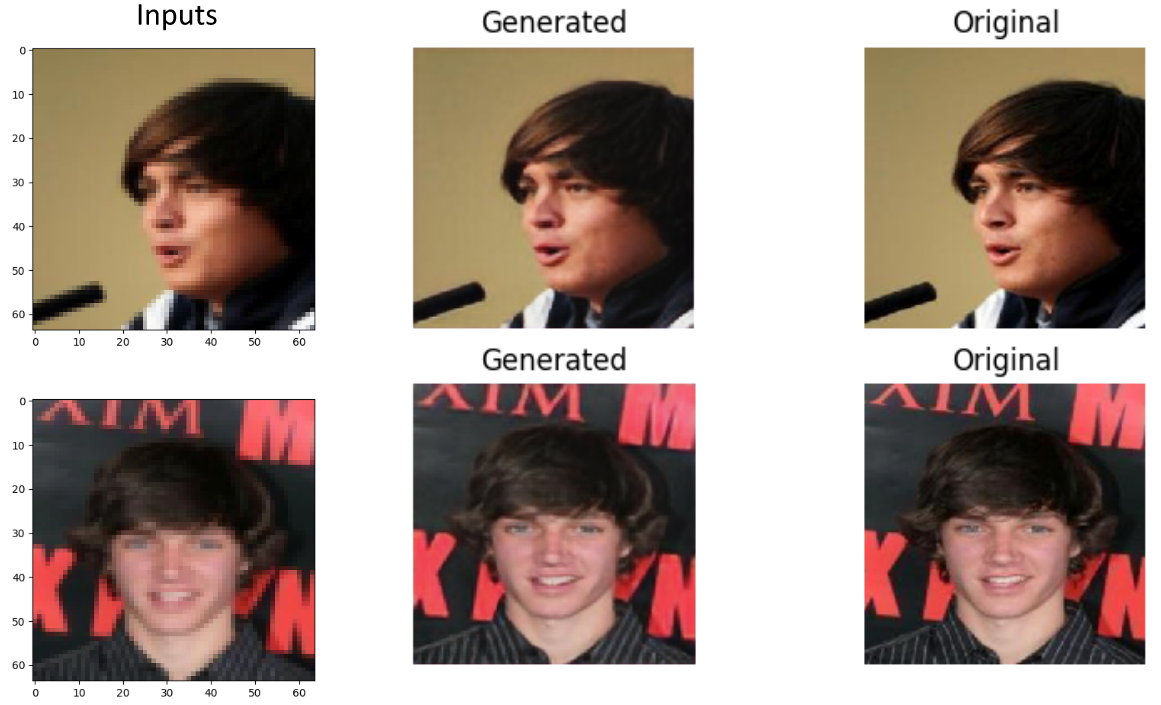
\includegraphics[width=0.45\textwidth]{images/gan-res.png}
	\caption{Results of the SRCGAN when run on the CelebA dataset after 6900
	iterations. The images on the left are the inputted images, alongside class
	information, the images in the middle are generated images, and the image on
	the right are the ground truth}
	\label{fig:gan-res}
\end{figure}

The results for the SRCGAN are shown in \ref{fig:gan-res}. The specific model was
trained for 6900 iterations. As shown in the figure, the GANs tends to perform
well in creating an image which has similar semantics to the ground truth. In
fact, if one didn’t know about the existence of the ground truth, it is entirely
possible to believe that the generated image isn’t fake.

PSNR is what is planned to be used in the measuring the final performance of the
super-resolution algorithm. Unfortunately, at the time of writing this paper,
the technique wasn’t in a state to present the PSNR results. These results will
be available in the final iteration of this paper.

\subsection{Stitching}
Before undergoing image stitching, the subject images and background image are
all separated as individual images. An example of this separation is shown
below:

[BACKGROUND IMAGE]
[SUBJECT IMAGE X] [SUBJECT IMAGE X] [SUBJECT IMAGE X] ...

From here, PIL is used to take the subject images and place them in their
appropriate places on the background image. Their positions are determined from
data provided by the image segmentation algorithm that gives the (x,y)
coordinate of the specified subject image in the background image and the
original subject image’s height and width dimensions. This reconstruction
results in a single image, an example of which is demonstrated below:

[RECONSTRUCTED IMAGE]

Now that all the images are merged into one image, blurring along the shared
edges between the subject images and background image needs to be done to make
the entirety of the image look more natural. This is done using OpenCV’s image
blurring functionality with a blur radius of (WIDTH, HEIGHT). The blurring is
done in such a way as to make a smooth transition from the resolution of the
subject images to the resolution of the background image. An example of the
final product can be seen below:

[IMAGE]

More details about the results of the image stitching process will be available
in the final iteration of this paper.
